\chapter{Materiais e Métodos}

\section{Construção da Ferramenta}


Dois equipamentos comerciais foram utilizados para construção da ferramenta de coleta sincronizada: 
Mindwave Mobile II e o GP3; para a coleta de EEG e ET, respectivamente. O código de coleta que gera o dataset
multimodal foi construído em MATLAB, e o pré-processamento dos dados antes de serem \textit{inputs} no treinamento
de algoritmos no software Orange foi construído em Python. O presente capítulo irá apresentar os equipamentos de coleta
e o método adotado para construção da ferramenta. 

\subsection{Mindwave Mobile II}
O equipamento possui um eletrodo de coleta e um eletrodo de referência que ficam posicionados 
acima da sobrancelha esquerda e na orelha esquerda do participante, respectivamente. 
A posição do eletrodo de coleta em relação ao sistema de referência de posição de eletrodos (10-20), é o FP1, 
correspondendo a região Frontopolar 1. A coleta de dados do aparelho se dá por conexão via \textit{bluetooth} e 
funciona em computadores Mac, Windows ou celulares Androids ou iOS, disponíveis em um raio de 10 metros (informações do fabricante). 
Ele coleta ondas cerebrais variando entre 3 e 100Hz, com uma frequência de 512Hz (NeuroSky Inc., 2015). 

O aparelho automaticamente distingue os dados coletados em ondas alfa, beta, gama, teta e delta; 
além de coletar informações subjetivas no formato de medidas de atenção e meditação, 
por meio de um algoritmo de reforço de aprendizado não disponibilizado ao publico. 
Também mede a ativação muscular próxima ao eletrodo para estimar a qualidade do sinal. 
O MindWave Mobile filtra interferência elétrica e converte o sinal detectado pelo eletrodo em sinal digital. 
O chip que faz o filtro e conversão se chama ThinkGear, e permite a filtragem de ruído para interferência ativação muscular (EMG) e 50/60Hz de corrente alternada. 

\begin{figure}
    \centering
    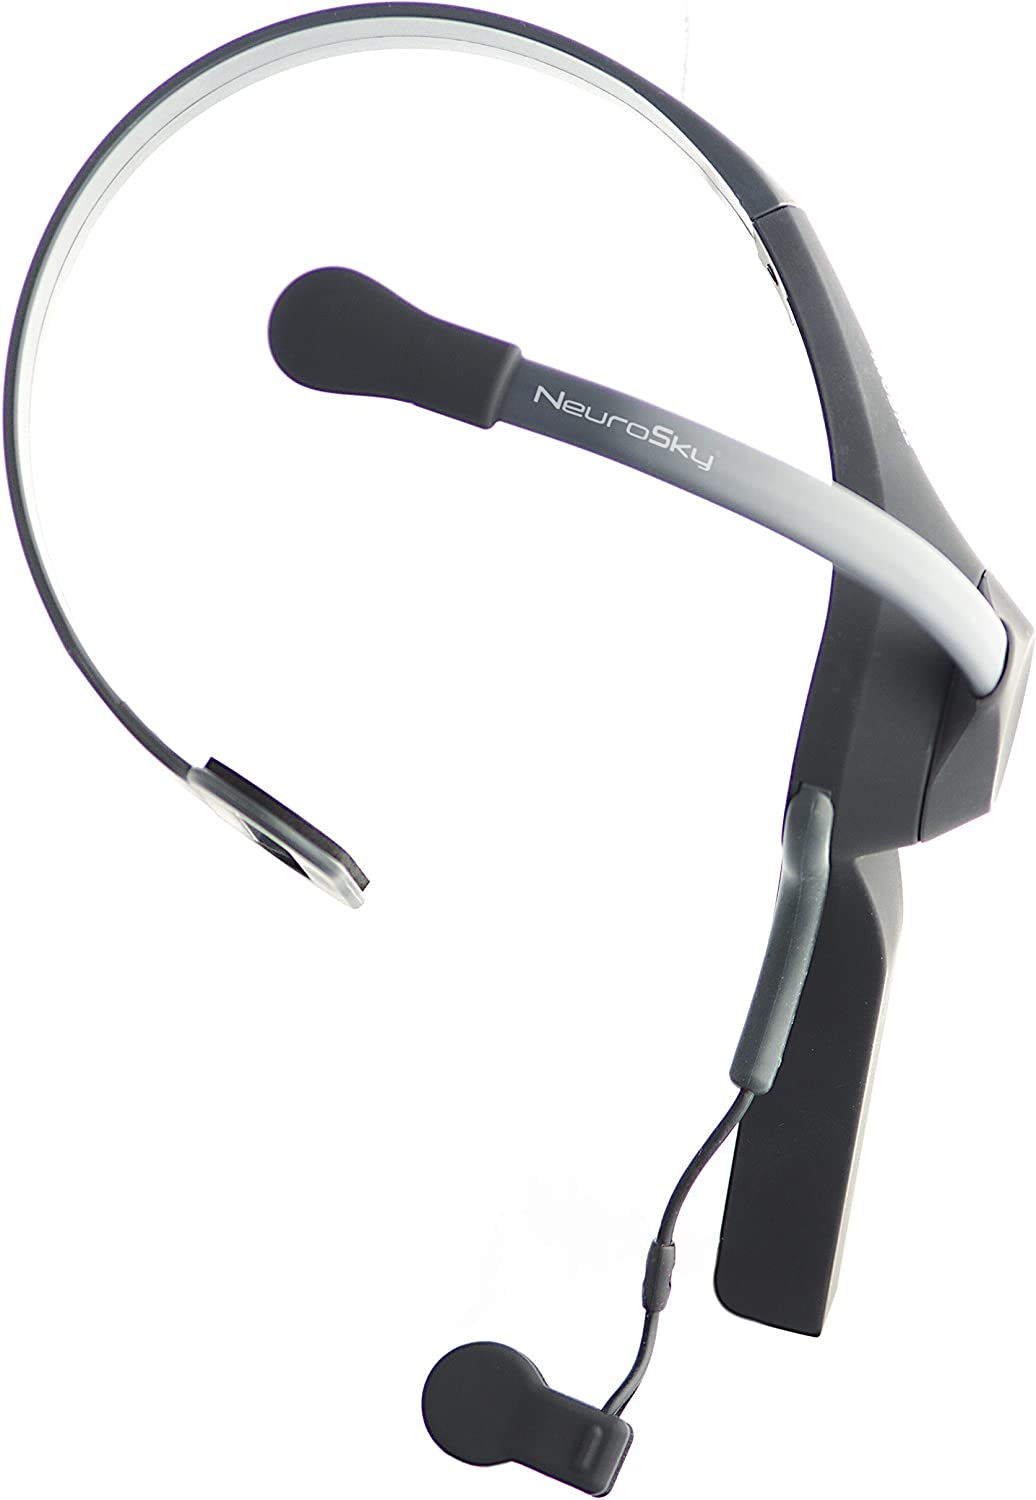
\includegraphics[width=40mm]{mindwave_II.jpg}
    \caption{Mindwave Mobile II (Neurosky)}
\end{figure}

Para o funcionamento adequado do Mindwave, é necessário instalar uma tecnologia 
chamada \textit{ThinkGear} (TG), que permite a troca de informações entre o equipamento 
e os softwares compativeis e processa o sinal detectado pelo eletrodo. 


\subsection{Gazepoint GP3}

O GP3 é um equipamento comercial de coleta do movimento dos olhos, 
fabricado pela Gazepoint. Possui software próprio para análise dos dados, 
além de ser possível realizar coleta de dados com linguagens de programação open-source. O GP3 funciona emitindo uma luz infravermelha (IR) 
diretamente nos olhos do participante e captando a reflexão da luz para localizar o ponto focal ao longo do tempo. 
Permite coletar a direção do olhar, número de fixações, tempo até a primeira fixação, taxa de piscadas,
 duração de piscadas, diâmetro da pupila, tempo de duração do olhar em um determinado ponto focal, 
 objetos observados em uma imagem, entre outros (informações do fabricante).

O Gazepoint GP3 estabelece sua conexão com o computador através de dois cabos USB - um cabo de energia e outro para dados.
Seu posicionamento ideal é logo abaixo do monitorde estímulo. Para um melhor posicionamento, o fabricante 
sugere uma distância ideal de 65 cm dos olhos do participante até o equipamento. O GP3 possui as seguintes características, conforme
especificado pelo fabricante:

\begin{itemize}
    \item Acurácia de 0.5-1 grau de ângulo visual
    \item 60 Hz de frequencia de atualização
    \item calibração de 5 e 9 pontos
    \item API
    \item Captura movimento de 25cm horizontais e 11cm verticais
    \item 15 cm de limite de profundidade de movimento
\end{itemize}

\begin{figure}
    \centering
    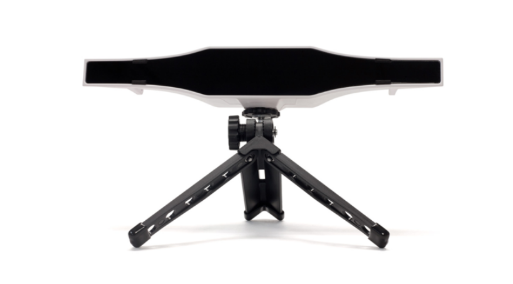
\includegraphics[width=100mm]{gp3.png}
    \caption{GP3 (Gazepoint)}
\end{figure}

A calibração é realizada pelo Gazepoint Control, afim de estabelecer qual o apontamento ocular do participante. 
A calibração pode ser feita em 5 pontos ou 9 pontos no monitor de exibição de estímulo. Os pontos na tela são apresentados
em sequencia e o participante deve acompanha-los com o olhar até a finalização da calibração. Após a calibração ser concluída, a API calcula o erro do sistema em relação ao olhar para o olho esquerdo (em verde) 
e direito (vermelho), dos pontos apresentados na tela. 

O  equipamento GP3 possui uma \textit{Application Programming Interface} (API) própria, 
o Open Gaze API. 
A API é uma alternativa de se controlar o equipamento sem precisar do software 
pago tambem feito pela Gazepoint. A API utiliza de um \textit{Transmission Control Protocol – Internet Protocol (TCP/IP) 
socket}, que permite a comunicação entre a aplicação e o servidor (fonte dos dados de ET). 
O IP determina o endereço para o qual os dados serão enviados, e o TCP utiliza a arquitetura de 
rede para realizar o transporte. O formato de dado utilizado para a API é o \textit{Extensible Markup Language} (XML), 
que também pode ser implementado e estabelecer conexão com Python. 
As portas utilizadas para a comunicação de forma padrão são: 
localhost (127.0.0.1) e port 4242. 


Na API do Gazepoint, o cliente tem duas tags de comunicação: GET e SET. 
Ao utilizar o SET o cliente pode alterar o valor de alguma variável. 
O comando GET não tem a possibilidade de alterção de valores. O servidor 
pode enviar dados para o cliente com diferentes tags: ACK, NACK, CAL e REC. 
As duas primeiras são geradas em resposta aos comandos de GET e SET (ACK – Sucesso e NACK –Falha). 
Os CAL são gerados com bases nas calibrações e REC serve para os dados gravados. 
Estas regras de escrita são utilizadas pelo codigo em Python para estabelecer o controle do GP3,
 permitindo que o código calibre o equipamento e estabeleça definições de variáveis.


\section{Linguagens de Programação e Softwares}


Para a análise de dados coletados, foram necessários a utilização de alguns
softwares. A escolha dos softwares foi dada com foco em um uso menos programático
(fácil usabilidade mesmo para pessoas com pouco conhecimento de programação) 
e disponibilidade de pacotes de interesse para as análises.

\subsection{Orange}
Orange é um software desenvolvido pela Universidade de Ljubljan (Demsar et
al., 2013), que permite a construção facilitada de pipelines de modelagem através de
click-and-point. Este software possibilita o estudo de diferentes algoritmos ao mesmo
tempo, incluindo análise das principais métricas de desempenho. O pipeline todo
pode ser montado com click-and-point, ou seja, sem precisar de programação.

\subsection{Python}
Python é uma linguagem de programação que vem crescendo seu uso na
atualidade. Por ser fácil de se interpretar e por sua ativa comunidade de
colaboradores, se faz uma linguagem de bastante interesse para a construção de
soluções de análises que englobam a academia e a indústria. Python é uma linguagem
criada com base em colaboração e sem custo. Logo, ao utilizarmos Python como
linguagem de desenvolvimento de solução, podemos reduzir o custo geral da
pesquisa.

\subsection{MATLAB}
O MATLAB é um software e linguagem de programação e software (Mathworks, 2018). A linguagem é baseada em matrizes e possibilita formas de visualizar
problemas complexos. Tem diversas “toolboxes”, que permite robustez e capacidade
de processamento para diferentes tipos de dados.

\section{Protocolo de Coleta}

Para a coleta simultânea, duas linguagens de programação foram utilizadas: MATLAB e Python, como tambpém 
utilizado no trabalho de Notaro et al. (2018).  
A montagem do \textit{setup} foi feita com base nas coletas realizadas para a construção dos datasets EEGEyeNet e 
ZuCO (Kastrati et al., 2021; Hollenstein et al., 2019), com o gazepoint a frente do monitor de exibição de estímulos
e com a montagem do equipamento de EEG antes de começar a coleta. 

\subsection{Preparo de Coleta}
Inicialmente, o software Gazepoint Control foi ligado para rodar em  \textit{background} no computador. 
Em seguida, o Mindwave mobile II foi ligado e teve sua conexão \textit{bluetooth} estabelecida e 
verificada. A porta de conexão (porta COM) PC-Mindwave pode mudar, 
então foi verificado em qual porta foi estabelecida a conexão 
em todo início de nova coleta. Após a verificação da porta, foi 
observado se houve necessidade de alterar
este valor na variável do código. O Gazepoint ficou distante do participante até o
software próprio acusar distância ideal (sinalizado por um sinal verde no topo do 
software de regulação do equipamento, figura 7.1).
Para teste de coleta foram utilizados dois monitores: um para calibração e apresentação de imagens,
e outro para o desenvolvimento de código e testagem (figura 7.2). 

Com o posicionamento do participante em frente as cameras, o passo de coleta dos dados deve ter início. 

\begin{figure}[!h]
    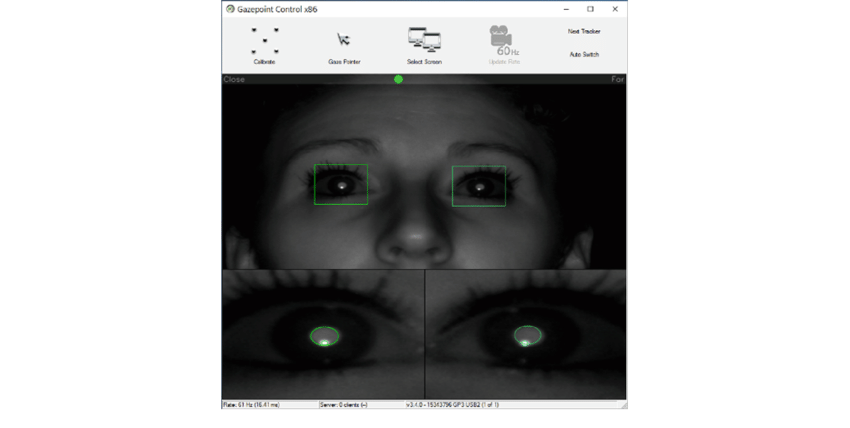
\includegraphics[width=200mm]{Gazepoint-GP3-setup-screen-showing-a-user-correctly-positioned-in-the-cameras-view-and.png}
    \caption{Exemplo do Opengaze conectado. Fonte: Sibley et al. (2017)}
\end{figure}



\begin{figure}
    \centering
    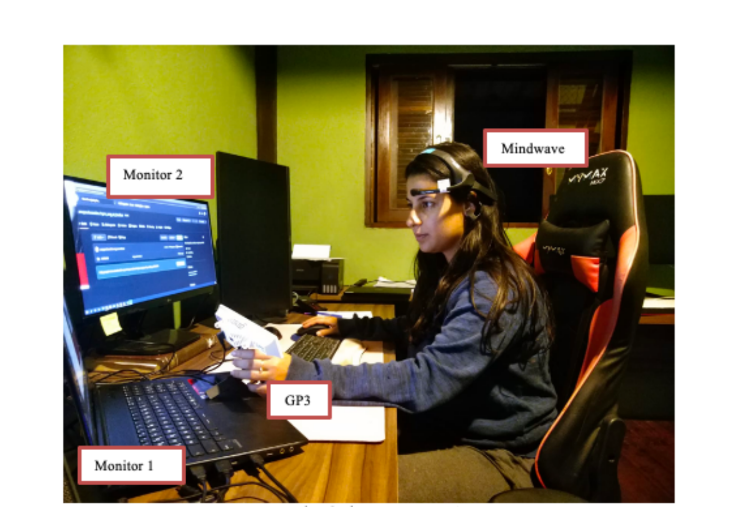
\includegraphics[width=150mm]{Screen Shot 2022-08-14 at 00.54.17.png}
    \caption{Montagem de Estudo de Caso da Ferramenta de Coleta EEG-ET.}
\end{figure}



%Tabela 6.1 Caracteristicas Montior utilizado na Coleta de Eye Tracking 
%Monitor	Video Interno conectado a Intel® HD Graphics 630
%Resolução da área de trabalho	1920  x 1080
%Resolução do sinal ativo	1920  x 1080
%Taxa de atualização	60 Hz
%Intensidade de bits	6 bits
%Formato de cor 	RGB
%Espaço de cores	Alcance dinâmico padrão




\textbf{1. Coletando com MATLAB}

O código em questão já se encontra disponível no \href{https://github.com/anapaulasandes/ppgeb_masters}{Github}.
Depois de adicionar a pasta com o código no \textit{path} do MATLAB, o código de coleta é
iniciado. O código foi construído com base na \textit{toolkit} Gazepoint, da EmotionCognitionLab. 
Ele age da seguinte forma:

\b egin{enumerate}
    \item Fecha todas as variáveis pré existentes;
    \item Estabelece conexão com o GP3;
    \item Executa a calibração do GP3 com 5 pontos em tela;
    \item Estabelece conexão com o TG do Mindwave Mobile II;
    \item Instancia um segundo terminal para envio de mensagens ao GP3 (mensagens enviadas são o valor do RAW do mindwave);
    \item Plota em tempo-real a visualização do plot de EEG;
    \item Fecha o segundo terminal após termino da coleta em tempo pré-determinado;
    \item Desconecta a conexão com ambos os equipamentos;
    \item Fecha o primeiro terminal instanciado.
\end{enumerate}

 A conexão com o GP3 é estabelecida no primeiro terminal. Como o GP3 permite 
 o envio de mensagens para o equipamento através da coluna USER, na presente solução ela é
 usada para armazenar as informações RAW do Mindwave mobile. As informações são escritas 
 pelo segundo terminal para o arquivo .txt (previamente definido no código). A captura de informações 
 do GP3 e Mindwave acontecem de forma imediatamente sucessiva. 